\hypertarget{_c_p_u_8cpp}{\section{Dokumentacja pliku /home/karolina/\-Pulpit/\-Project41\-Poker(1)/\-Project41\-Poker/\-Project41\-Poker/prj/src/\-C\-P\-U.cpp}
\label{_c_p_u_8cpp}\index{/home/karolina/\-Pulpit/\-Project41\-Poker(1)/\-Project41\-Poker/\-Project41\-Poker/prj/src/\-C\-P\-U.\-cpp@{/home/karolina/\-Pulpit/\-Project41\-Poker(1)/\-Project41\-Poker/\-Project41\-Poker/prj/src/\-C\-P\-U.\-cpp}}
}


Definicja metody klasy \hyperlink{class_c_p_u}{C\-P\-U}.  


{\ttfamily \#include \char`\"{}C\-P\-U.\-h\char`\"{}}\\*
{\ttfamily \#include $<$ctime$>$}\\*
Wykres zależności załączania dla C\-P\-U.\-cpp\-:\nopagebreak
\begin{figure}[H]
\begin{center}
\leavevmode
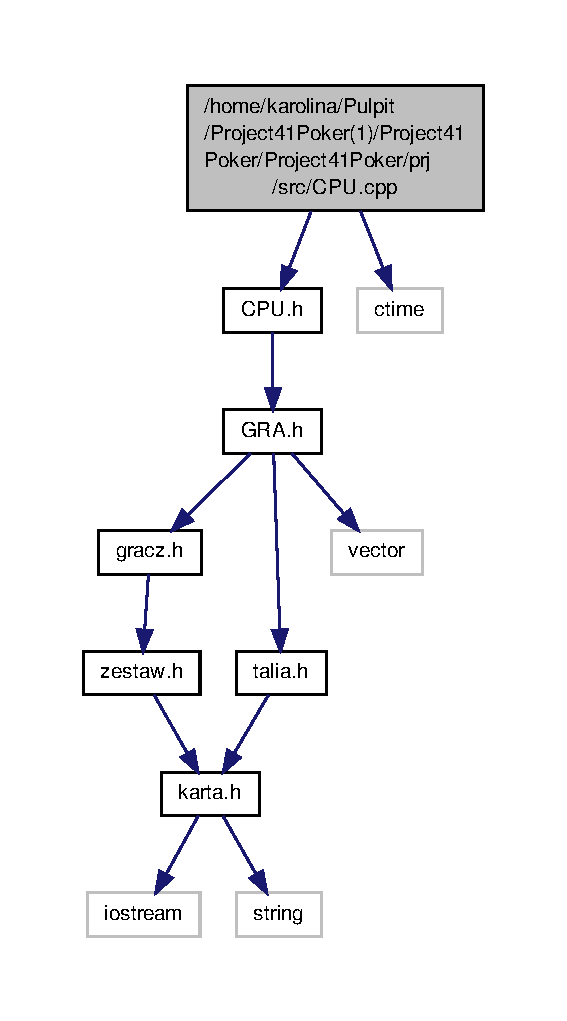
\includegraphics[width=272pt]{_c_p_u_8cpp__incl}
\end{center}
\end{figure}


\subsection{Opis szczegółowy}
Zawiera definicje metod klasy \hyperlink{class_c_p_u}{C\-P\-U}. 

Definicja w pliku \hyperlink{_c_p_u_8cpp_source}{C\-P\-U.\-cpp}.

